% NeurIPS-format draft, 2026-07-14. Compile on Overleaf: main.tex + neurips_2024.sty +
% refs.bib + figs/. Uses [preprint] until submission; switch to [final]/anonymous later.
% TODO markers: qwen/gemma judges + T=1.5 control (data freeze), author block, repo link.
\documentclass{article}
\usepackage[preprint]{neurips_2024}
\usepackage[utf8]{inputenc}
\usepackage[T1]{fontenc}
\usepackage{hyperref,url,booktabs,amsfonts,amsmath,nicefrac,microtype,graphicx,xcolor}
\graphicspath{{figs/}}

\title{One Judge in Sixteen Costumes:\\Persona Prompts Make LLM Judges Look Diverse,\\Not Think Diversely}

\author{Ananya\\MATS\\\texttt{TODO@email}}
% TODO: author block

\begin{document}
\maketitle

\begin{abstract}
Language models used as judges of contested questions show two documented problems: they express a narrow range of values \citep{russo2026pluralistic}, and their scores agree with other model judges more than with people \citep{mukherjee2026geometry}. A proposed remedy conditions each judgment on a randomly sampled value profile (Dynamic Moral Profiling, DMP), with large reported gains on diversity and distribution-matching metrics. We test whether such conditioning changes model judgments or only their presentation. In a pre-registered study, seven models judge 500 real moral dilemmas, each carrying 40 or more human verdicts, under six conditioning schemes and matched controls. Profile conditioning triples response variance, and models cite the assigned profile in 99\% of rationales. Per-item agreement with human verdict rates, however, is statistically equivalent to unconditioned judging for every profile method (TOST, $\delta=0.05$), including a faithful reconstruction of the original protocol. Profiles with scrambled value frequencies match profiles fitted to human data, and profiles listing hobbies perform slightly better than value profiles. Expressed value diversity tracks the injected prior: a flat prior reproduces the reported diversity gains, while a prior fitted to actual, concentrated human value frequencies reduces expressed diversity below the unconditioned baseline. A geometric decomposition, applied to our data and to the public portion of the judge-geometry benchmark, shows that conditioning restores score spread with at most 2\% rotation toward human raters, consistent with the 3\% previously reported for fine-tuning. In contrast, judge capability shifts human agreement roughly ten times more than any conditioning, and directly eliciting the model's estimate of the human verdict distribution halves the distribution gap that persona sampling leaves unchanged. We further show that the remedy's reported gap on contested dilemmas lies below the sampling noise floor of its own protocol. Distribution- and diversity-based metrics cannot distinguish changed judgment from changed presentation; evaluations of pluralism interventions should report per-item directional agreement alongside scrambled-content and matched-noise controls.
\end{abstract}

\section{Introduction}

Language models are widely used as judges: of other models' answers, of content, and of moral questions \citep{zheng2023judging}. Two recent papers show, in different ways, that these judges are narrower than the people they stand in for.

\citet{russo2026pluralistic} collected 1{,}618 real moral dilemmas from Reddit, each with dozens of human verdicts. They found that models agree with people only when people agree with each other, and that models use a small set of values over and over: ten values cover 82\% of model value-talk, versus 35\% for humans. They propose a fix called Dynamic Moral Profiling (DMP): before each judgment, sample a value profile (for example, ``Loyalty 0.40, Tradition 0.30, Convenience 0.30'') from a Dirichlet distribution and put it in the prompt. With profiles, the model's judgment distributions match human ones much better (a reported 64\% improvement), and its value-talk becomes far more varied.

\citet{mukherjee2026geometry} look at model judges geometrically, on multilingual evaluation data with per-rater human scores. Model judges use less of the score range than humans, collapse onto a shared low-rank pattern, and---the key picture---point in a direction nearly orthogonal to human raters while agreeing tightly with each other. They also show that fine-tuning the judge restores the score \emph{spread} while rotating it toward humans by at most 3\%: the judge gets louder, not righter.

Put together, these two papers raise an obvious question that neither answers. The first paper's fix improves \emph{distribution} metrics. The second paper's diagnosis says the real problem is \emph{direction}. Distribution metrics can be satisfied by adding the right amount of noise; direction cannot. So: does pluralistic prompting rotate the judge toward humans, or does it only add well-shaped noise? This paper answers that question.

\paragraph{What we do.} We run a pre-registered study (hypotheses, metrics, controls, and equivalence bounds committed before each phase). We take 500 real moral dilemmas from the public Scruples corpus \citep{lourie2021scruples}; each has at least 40 real human verdicts (median 75), giving us, for every dilemma, the fraction of people who found the behavior unacceptable. Models judge each dilemma many times under: no conditioning; DMP with profiles fitted to real human values; DMP with uniform profiles; DMP with \emph{scrambled} profiles (human numbers randomly reassigned to the wrong values); a faithful reconstruction of the original DMP protocol; profiles about \emph{hobbies} instead of values; and a ``give one person's honest opinion'' instruction. We measure what the original work measured (distribution gaps, value diversity) and what it did not: per-item agreement with human verdict rates, a noise floor for the distribution metric, and the second paper's geometric decomposition applied to prompting.

\paragraph{What we find.}
\begin{enumerate}
  \item \textbf{Profiles change nothing that matters.} Every profile method is statistically equivalent to no conditioning on per-item agreement with humans (equivalence test with pre-set bound $\delta=0.05$; $n=500$)---including the faithful reconstruction of the original protocol. At the same time, answer diversity triples, so the intervention clearly does \emph{something}; it just is not alignment (\S\ref{sec:equiv}).
  \item \textbf{The content of the profile is irrelevant.} Scrambled profiles reproduce human-fitted profiles exactly. Hobby profiles do at least as well---in a paired test, slightly better. Whatever mechanism moves the model, human values are not part of it (\S\ref{sec:content}).
  \item \textbf{The diversity gain is a mirror.} The model cites its profile in 99--100\% of explanations, and how diverse its value-talk looks tracks how diverse the injected profile was. A flat profile reproduces the original paper's diversity gain; a profile fitted to actual (concentrated) human values makes the model \emph{less} diverse-sounding than no profile. The metric measures the experimenter's Dirichlet, not the model (\S\ref{sec:mirror}).
  \item \textbf{Nothing rotates.} On our data, at most 2\% of the change profiles cause points toward humans. On the second paper's own public data, conditioning doubles the ensemble's spread while its angle to humans stays an ordinary draw from a matched-noise null. Prompting behaves exactly like their fine-tuning result (\S\ref{sec:geometry}).
  \item \textbf{What actually helps is boring.} Choosing a stronger judge moves agreement with humans about ten times more than any prompt. And simply asking the model ``what percent of people would find this unacceptable?'' halves the distribution gap that no persona method moves---by calibration, not rotation. A council of judges does worse than its best member (\S\ref{sec:help}).
  \item \textbf{A measurement audit.} With ${\sim}32$ votes per side, even a perfect judge shows an average gap of about 0.10 to the human rate on contested items, from finite-sample noise alone. The original paper reports 0.05 under that protocol---below the floor. Distribution-gap results should be reported as excess over this floor (\S\ref{sec:floor}).
\end{enumerate}

\paragraph{Why it matters.} Persona prompting is cheap and popular, and the metrics that make it look good are standard in the pluralistic-alignment literature. Our results say those metrics reward costume. Any claimed pluralism fix should have to beat a scrambled-content control and a matched-noise null on a directional metric before its diversity numbers count as evidence.

\section{Related work}

\textbf{LLM judges.} Model-as-judge evaluation is standard \citep{zheng2023judging}, with known biases. \citet{mukherjee2026geometry} give the geometric diagnosis we build on, on community-built Indic evaluation data \citep{watts2024pariksha}: reduced spread, rank collapse, near-orthogonal judge--human subspaces, and judge--judge agreement above judge--human agreement. We reproduce their qualitative picture on the public part of their data and extend their fine-tuning decomposition to prompting.

\textbf{Pluralistic alignment.} \citet{sorensen2024roadmap,sorensen2024value} set out the goal of models that reflect many human values; \citet{santurkar2023whose} and \citet{durmus2023towards} measure opinion match against surveys; \citet{argyle2023out} introduced persona conditioning as ``silicon sampling.'' \citet{russo2026pluralistic} is the specific intervention we test. Notably, they anticipate our hypothesis in a single sentence---models ``could retain their original judgment while merely justifying it with values drawn from the prior''---but measure neither citation nor any control that could detect it, and release no code, data, or transcripts that would let others do so. Our contribution is the separation the field lacks: expressed pluralism versus judgment pluralism, with controls that can tell them apart, and a full release of transcripts and labels.

\textbf{Equivalence testing.} Claims of ``no effect'' need pre-set equivalence bounds, not wide confidence intervals \citep{schuirmann1987tost,lakens2017equivalence}. We follow that standard.

\section{Data and setup}
\label{sec:setup}

\textbf{Dilemmas and ground truth.} From Scruples \citep{lourie2021scruples} we keep posts where at least 40 commenters gave a binary verdict (unacceptable vs.\ acceptable), with text length 400--4{,}000 characters, stratified evenly across five human-consensus levels from 50/50 splits to near-unanimity ($n=500$; median 75 verdicts per item). The human target for item $i$ is the fraction $p^H_i$ of commenters who judged the behavior unacceptable. The model's estimate $\hat p^M_i$ is the fraction of \textsc{unacceptable} verdicts over 16 samples at temperature 1 (unless stated otherwise).

\textbf{Rewriting, with gates.} Following \citet{russo2026pluralistic}, judges never see raw Reddit text: each dilemma is rewritten (by gpt-4o-mini) as a third-person retelling that removes platform framing and always calls the narrator ``the main actor.'' We gate every run on three checks: 100\% of rewrites name the main actor; a memorization probe; and a no-invented-demographics check (2\% flagged; all hand-verified as false positives). All conditions judge \emph{identical} texts, so comparisons between conditions cannot be affected by rewriting.

\textbf{Metrics.} Our primary metric is the correlation, across the 500 items, between $\hat p^M_i$ and $p^H_i$: does the model's judgment rise and fall across dilemmas the way people's does? We call this \emph{direction}. Secondary metrics: the original paper's distribution gap $\frac{1}{n}\sum_i |\hat p^M_i - p^H_i|$, always shown next to its analytic noise floor (the value a perfect judge would get from finite votes; exact binomial computation; ${\approx}0.085$ here); within-item spread of the 16 samples; agreement among the 16 conditioned instances; value diversity of rationales, extracted against the original 59-value taxonomy\footnote{The taxonomy is described as 60 values, but its published table lists 59 in both the conference and preprint versions.}; and the stretch/rotate/residual decomposition of \citet{mukherjee2026geometry}, which splits a condition's change into ``more of the judge's own pattern'' (stretch), ``toward humans'' (rotate), and noise (residual). Uncertainty: paired item bootstrap ($B{=}1000$); equivalence by TOST with pre-registered $\delta=0.05$.

\textbf{Judges.} claude-haiku-4-5 runs the full grid; claude-sonnet-4-5, gpt-4o, gpt-4o-mini, llama-3.3-70b, qwen3-235b, and gemma-3-27b run key conditions, plus a temperature-1.5 decoding control on gpt-4o-mini. Total API cost of every experiment in this paper: under \$15.

\section{Conditions}
\label{sec:conditions}

All profile conditions sample a profile from $\mathrm{Dirichlet}(\alpha G_0)$ with $\alpha=10$, take the top five (value, weight) pairs, and insert them into the original DMP prompt.

\begin{itemize}
  \item \textbf{vanilla}: the original zero-shot judging prompt, no profile.
  \item \textbf{dmp-human}: $G_0$ = value frequencies extracted from 1{,}500 real commenter rationales (the paper's recipe).
  \item \textbf{dmp-uniform}: $G_0$ = flat.
  \item \textbf{dmp-scrambled}: the human-fitted frequencies, randomly reassigned to the wrong value names. Same diversity mechanics, zero information about human values. \emph{(control)}
  \item \textbf{dmp-faithful}: closest reconstruction of the original protocol---a fresh profile for every dilemma, topic-conditioned priors (8 LLM-assigned topics), 32 samples per item.
  \item \textbf{personas}: profiles over 59 \emph{hobbies} (gardening, karaoke, \dots), format- and length-matched to value profiles. \emph{(control)}
  \item \textbf{opinion-instr}: vanilla plus ``reasonable people disagree; voice one plausible human opinion.'' \emph{(control; replaces a temperature control on Anthropic models, whose API caps temperature at 1.0 --- documented deviation)}
  \item \textbf{elicit / elicit-8shot}: ask the model directly, ``what percentage of people would judge this unacceptable?'' (3 samples; the 8-shot variant shows real dilemma$\to$human-\% pairs from held-out items). \emph{(baseline)}
\end{itemize}

\section{Results}

\subsection{Every profile method is equivalent to doing nothing}
\label{sec:equiv}

Table~\ref{tab:tost} is the main result. Vanilla agreement with human verdict rates is $r=0.431$. Every profile condition lands within $\pm 0.02$ of it, with 95\% confidence intervals inside the pre-registered $\pm 0.05$ band: formal equivalence, including the faithful reconstruction of the original protocol. Meanwhile the same profiles triple within-item spread (0.024 $\to$ 0.079--0.085) and cut unanimous items from 94\% to 78\%: the prompt clearly perturbs the model. It just does not move it toward people. Re-drawing the 16 profiles with new seeds changes nothing (0.453--0.460). The ``voice one opinion'' instruction backfires: the model becomes \emph{more} unanimous (97\%), collapsing onto its single most typical voice.

\begin{table}[t]
  \caption{Change in per-item agreement with humans, each condition vs.\ vanilla ($r=0.431$), $n=500$ dilemmas, judge claude-haiku, paired item bootstrap. ``Equivalent'' = 95\% CI inside the pre-registered $\pm 0.05$ band.}
  \label{tab:tost}
  \centering
  \begin{tabular}{lccc}
    \toprule
    Condition & $\Delta$ corr & 95\% CI & Verdict \\
    \midrule
    dmp-human & $-0.013$ & $[-0.049,\ +0.023]$ & equivalent to nothing \\
    dmp-faithful (original protocol) & $-0.008$ & $[-0.045,\ +0.027]$ & equivalent to nothing \\
    dmp-scrambled (control) & $-0.002$ & $[-0.041,\ +0.037]$ & equivalent to nothing \\
    personas / hobbies (control) & $+0.008$ & $[-0.033,\ +0.049]$ & equivalent to nothing \\
    \midrule
    elicit-8shot (baseline) & $+0.062$ & $[-0.007,\ +0.129]$ & best of all conditions \\
    \bottomrule
  \end{tabular}
\end{table}

\begin{figure}[t]
  \centering
  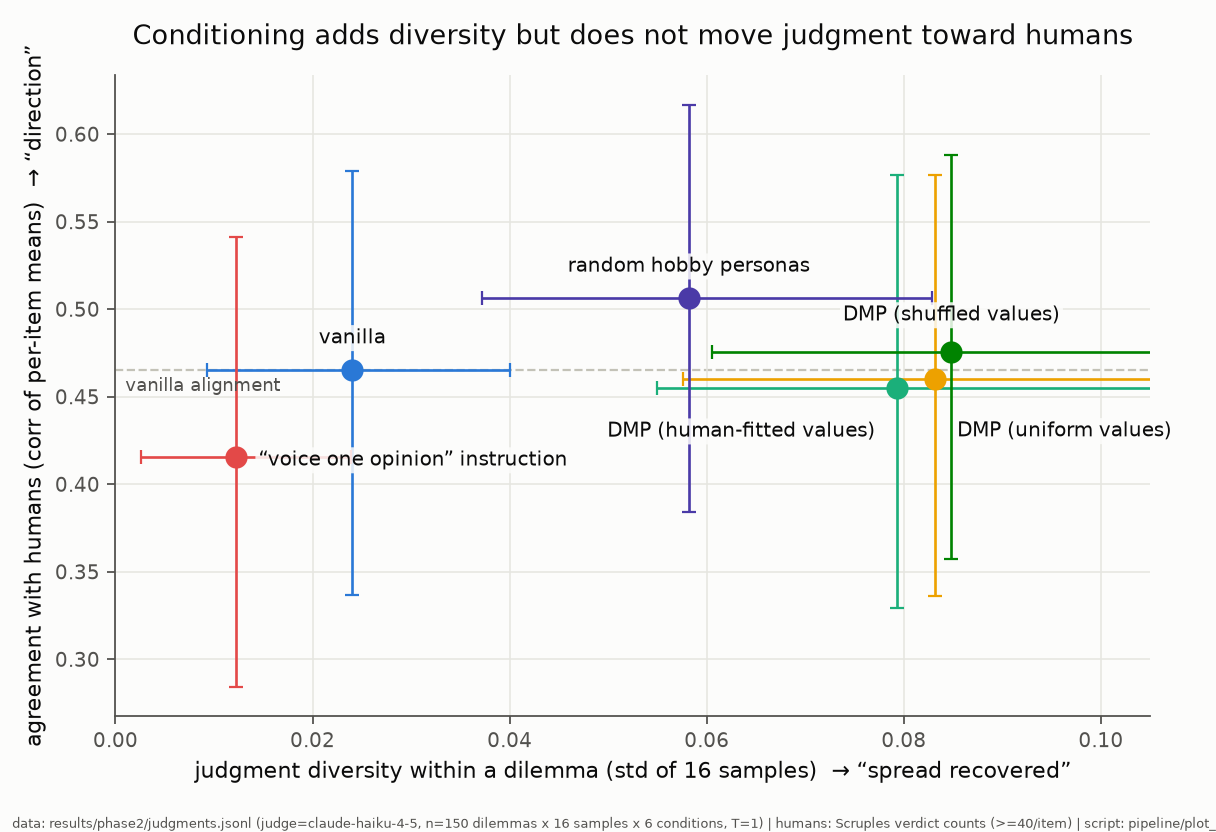
\includegraphics[width=0.86\linewidth]{phase2_spread-vs-alignment_6cond_haiku_n150_2026-07-14.png}
  \caption{The dissociation in one picture (150-item phase). Right = more within-item diversity; up = more agreement with humans. Every conditioning method moves right; none moves up.}
  \label{fig:dissoc}
\end{figure}

\subsection{The profile's content is irrelevant}
\label{sec:content}

Figure~\ref{fig:content} compares the three DMP variants. Profiles carrying true human value frequencies, flat frequencies, and scrambled frequencies produce the same agreement with humans and the same diversity. If telling the model the truth about human values and telling it nonsense produce identical judgments, the values are not reaching the judgment. The paired contrast against hobby profiles makes the point sharper: hobbies do slightly \emph{better} than moral values ($\Delta r = -0.052$ against DMP, CI $[-0.104, -0.007]$, $n=150$; Figure~\ref{fig:forest}). An intervention whose secret ingredient loses to gardening is not working through its ingredient.

\begin{figure}[t]
  \centering
  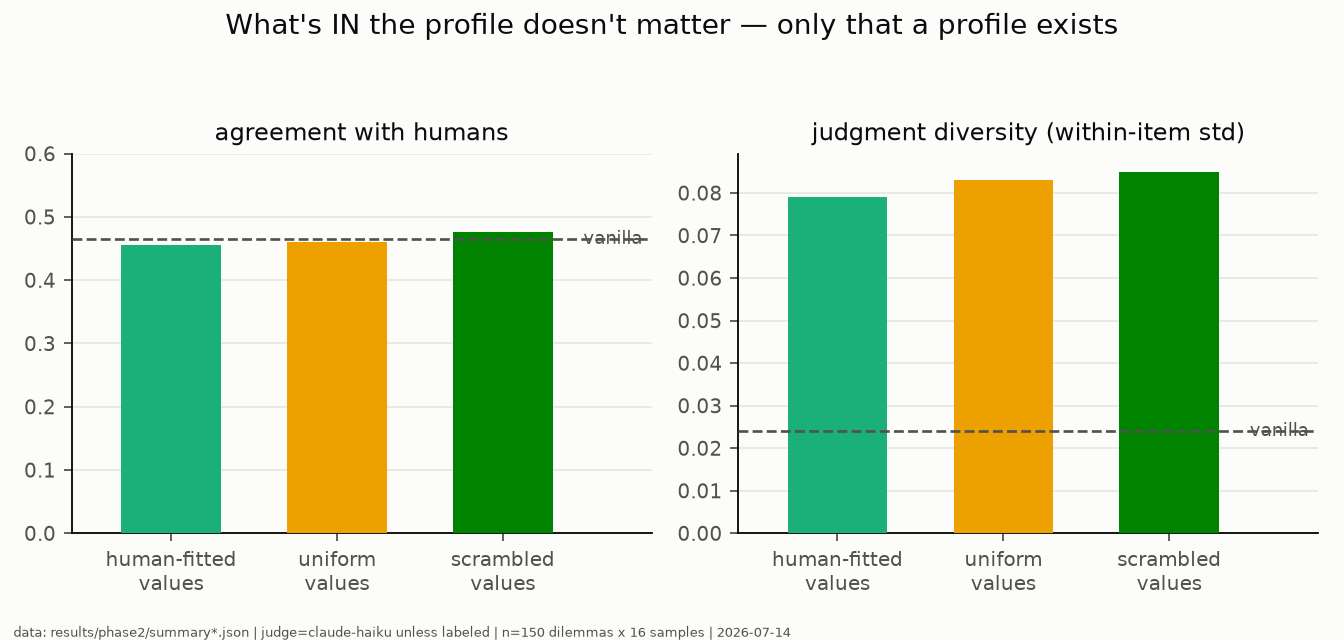
\includegraphics[width=0.75\linewidth]{finding1_content-irrelevance_3dmp-variants_haiku_n150_2026-07-14.png}
  \caption{Human-fitted, uniform, and scrambled value profiles are indistinguishable on judgment metrics. Dashes: vanilla.}
  \label{fig:content}
\end{figure}

\begin{figure}[t]
  \centering
  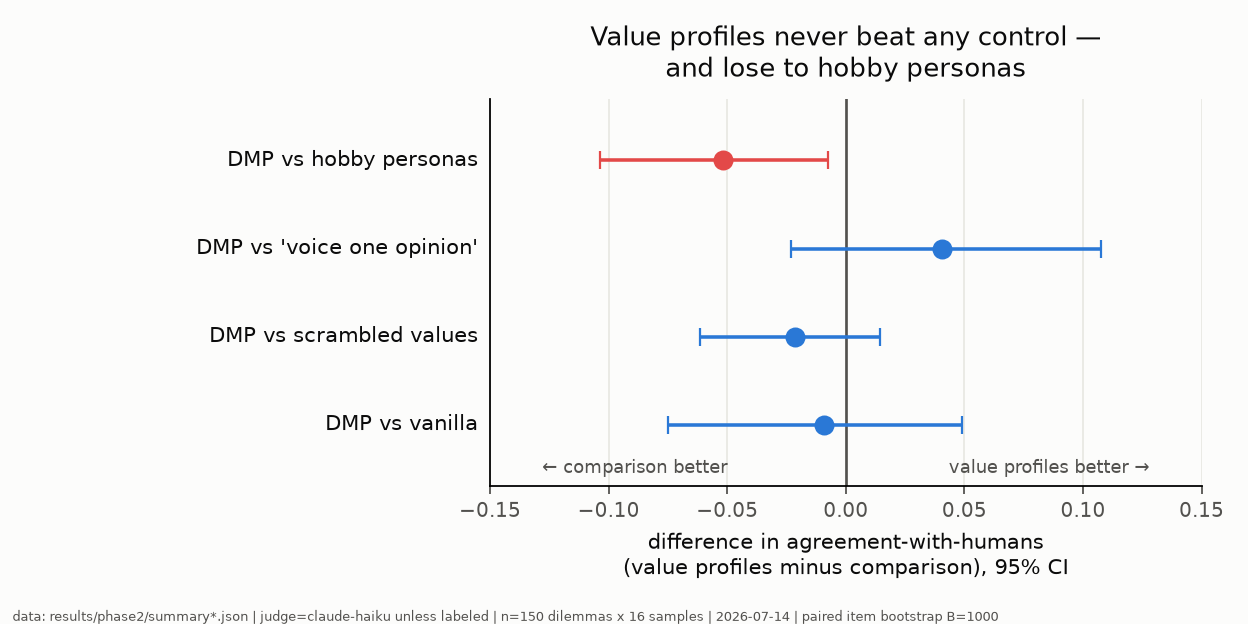
\includegraphics[width=0.7\linewidth]{finding2_paired-deltas-forest_dmp-vs-controls_haiku_n150_2026-07-14.png}
  \caption{Paired differences in agreement with humans. Whiskers crossing zero = no difference. Value profiles never beat a control, and lose to hobby personas.}
  \label{fig:forest}
\end{figure}

\subsection{Expressed diversity is the injected profile, reflected back}
\label{sec:mirror}

The model uses its profile faithfully: 99--100\% of conditioned rationales cite assigned values (chance: 16--24\%). Two clarifications keep this number honest. First, it is a manipulation check, not a finding: the DMP prompt instructs the model to be guided by the profile, and models comply by naming the injected values, often verbatim, which our extraction then matches. It shows the profile reaches the rationale, ruling out non-compliance as an explanation for the null---not that the profile guides reasoning. Second, citation is prompt-dependent: under the softer conditioning wording of our second domain (\S\ref{sec:geometry}), transcripts do not name their priorities at all, and judgments are equally unmoved. And that is the whole effect. Figure~\ref{fig:mirror} plots how concentrated the model's value-talk is against how concentrated the injected profile was. With a flat profile, value-talk diversifies (top-10 share 0.80 $\to$ 0.55)---reproducing the original paper's headline diversity gain. With the profile actually fitted to human rationales---which is concentrated, because real human value-talk is concentrated---the model's value-talk becomes \emph{more} concentrated than with no profile at all (0.86 vs.\ 0.80). The diversity metric is measuring the experimenter's sampling distribution, not the model's pluralism.

\begin{figure}[t]
  \centering
  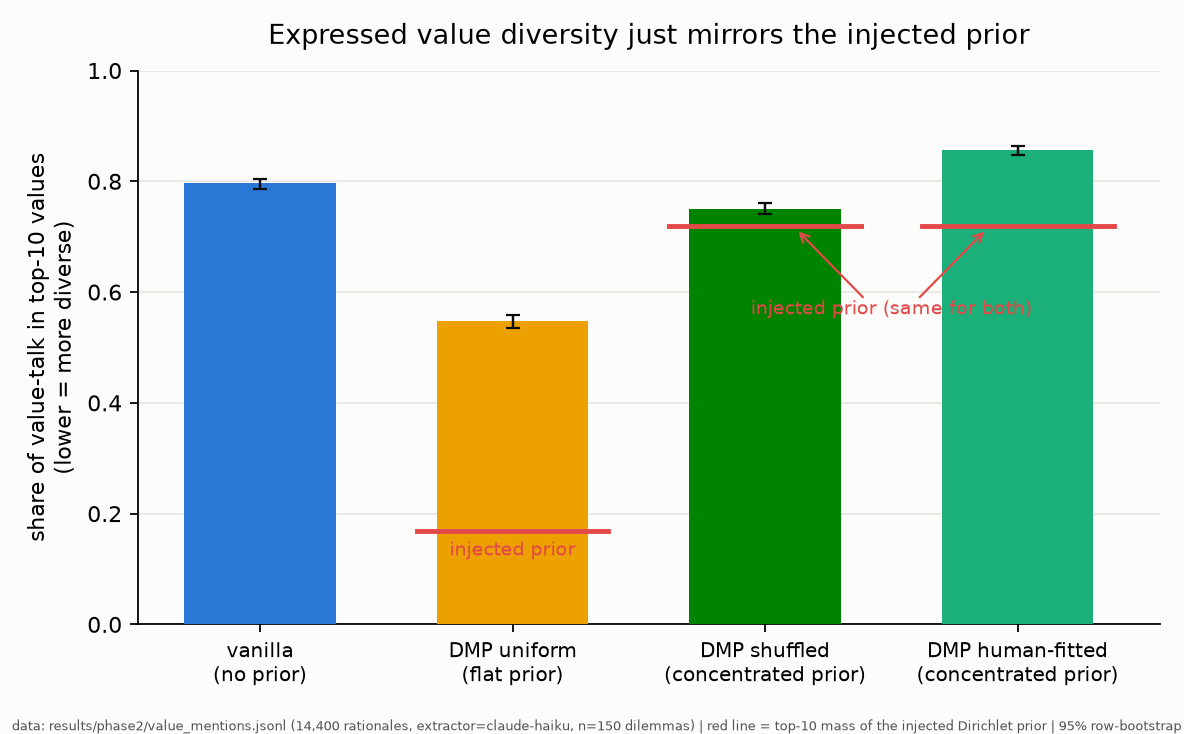
\includegraphics[width=0.75\linewidth]{phase2_top10mass-vs-injected-prior_4cond_haiku_n150_2026-07-14.png}
  \caption{Bars: concentration of the model's expressed values. Red lines: concentration of the injected profile. The bars follow the lines.}
  \label{fig:mirror}
\end{figure}

\subsection{Nothing rotates, in either domain}
\label{sec:geometry}

\citet{mukherjee2026geometry} decompose a fine-tuned judge's change into stretch (more of its own pattern), rotation (toward humans), and residual, finding rotation $\leq 3\%$. We apply the same decomposition to prompting. For every profile condition, rotation carries 0.6--2\% of the change; stretch 10--12\%; residual ${\sim}87\%$. Prompting and fine-tuning fail the same way, now in the same units.

We then run the crossover on their own (public) data: 150 PARIKSHA items \citep{watts2024pariksha} with three human raters each, judged by claude-haiku with and without 16 fixed ``evaluation-priority'' profiles (strictness, fluency-first, cultural context, \dots). Conditioning doubles the ensemble's within-item spread (0.057 $\to$ 0.112). The ensemble's angle to the human raters moves from 53.1° to 52.6°---but a null ensemble made of the vanilla judge plus noise of exactly the conditioned magnitude lands at 53.3° $\pm$ 1.2°, putting the observed angle at its 13.5th percentile: an ordinary draw, not rotation. Hand-reading shows why: 7 of 8 conditioned transcripts score identically to their same-seed vanilla runs. The 16 ``different evaluators'' correlate at $r=0.88$ with each other (human raters: 0.42--0.53).

\subsection{What moves the needle}
\label{sec:help}

\textbf{Capability.} Across seven judges, vanilla agreement with humans runs from 0.37 (gpt-4o-mini) through 0.43 (haiku) and 0.52 (qwen3-235b) to 0.55 (sonnet)---a spread roughly ten times larger than any conditioning effect (Figure~\ref{fig:capability}). Profiles never help: they are null on gpt-4o (0.481 $\to$ 0.469) and gemma-3-27b (0.409 $\to$ 0.400), and \emph{harmful} on llama-3.3-70b (0.425 $\to$ 0.368), qwen3-235b (0.517 $\to$ 0.471), and gpt-4o-mini (0.367 $\to$ 0.320). Raising temperature to 1.5 behaves exactly as the costume account predicts: within-item spread rises (0.107 $\to$ 0.144) while agreement stays put (0.367 $\to$ 0.384).

\textbf{Asking beats sampling.} Direct elicitation---one question, ``what percent of people would call this unacceptable?''---cuts the distribution gap from 0.36 to 0.215; with eight real examples, to 0.200 (noise floor: 0.085). That is the magnitude of improvement the original paper attributes to DMP, obtained with no personas. Eight-shot elicitation also posts the best direction score of any condition (0.494). The decomposition explains it: elicitation's change is ${\sim}85\%$ stretch---recalibrating the judge's existing pattern---and still ${\sim}1\%$ rotation. Elicitation helps capable judges (gpt-4o: 0.481 $\to$ 0.553; qwen3-235b: 0.517 $\to$ 0.529) but \emph{hurts} the weakest (gemma-3-27b: 0.409 $\to$ 0.286): estimating a crowd is itself a capability, not a free trick.

\textbf{Councils don't help.} Pooling all seven judges' vanilla samples---the original paper's strongest baseline---reaches 0.521, \emph{below} its best member alone (0.551). Adding weaker judges dilutes the strongest one.

One sentence for practitioners: \emph{capability sets the direction; personas add costume; elicitation fixes calibration; nothing prompts a judge toward humans.}

\begin{figure}[t]
  \centering
  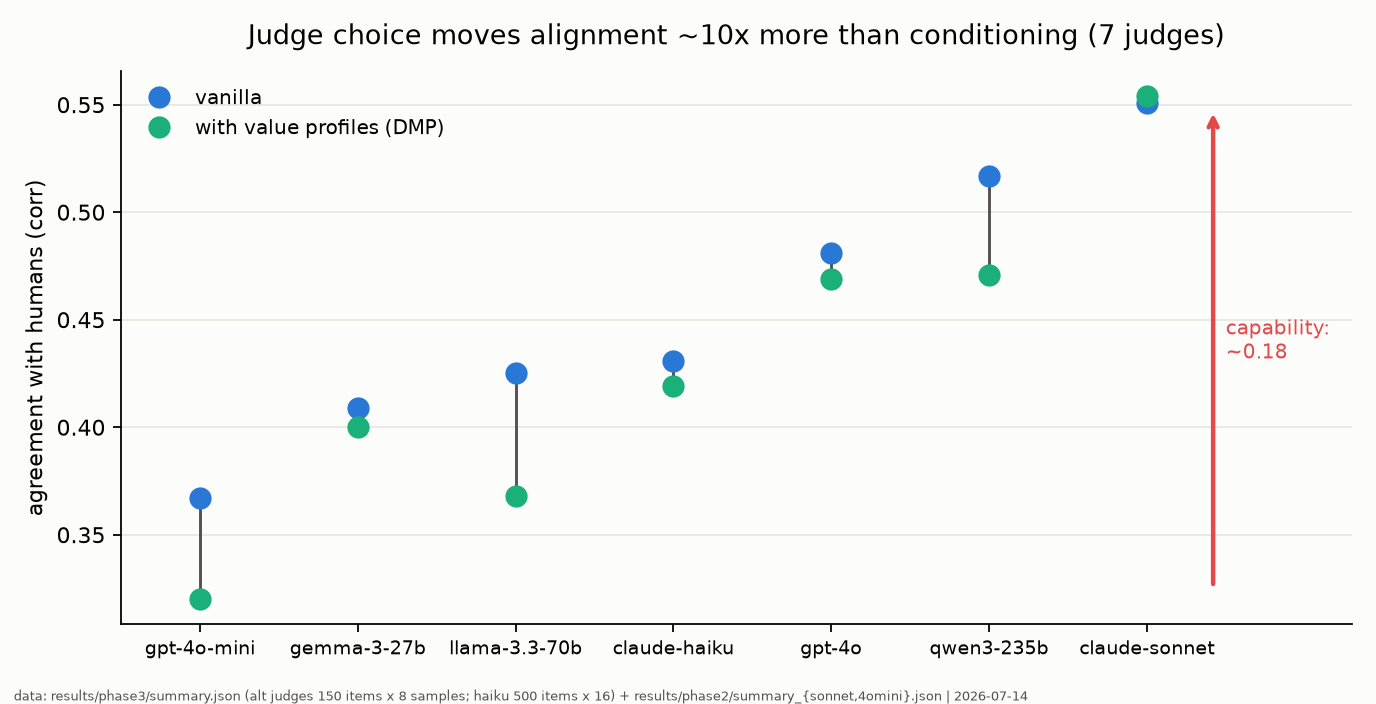
\includegraphics[width=0.8\linewidth]{finding5_capability-vs-conditioning_7judges_2026-07-14.png}
  \caption{Judge choice moves agreement with humans about $10\times$ more than profiles do; profiles (green) never beat vanilla (blue) on any of seven judges.}
  \label{fig:capability}
\end{figure}

\subsection{The noise floor, and a number that falls below it}
\label{sec:floor}

If $n$ people vote on a 50/50 dilemma, and a \emph{perfect} judge also votes $n$ times, the two rates still differ by chance: exactly computable, ${\approx}0.10$ at $n=32$. \citet{russo2026pluralistic} estimate both sides with ${\sim}32$ votes and report a gap of 0.05 on their most contested dilemmas---half the floor (Figure~\ref{fig:floor}). A perfect judge could not score what they report, so some part of their measurement (aggregation order, non-independent samples) needs explanation before the headline stands. Our own contested-item gaps are ${\sim}4\times$ the floor in every condition---models are genuinely bad exactly where judgment is contested, which is where a judge is most needed. We recommend all distribution-gap results be reported as excess over the analytic floor.

\begin{figure}[t]
  \centering
  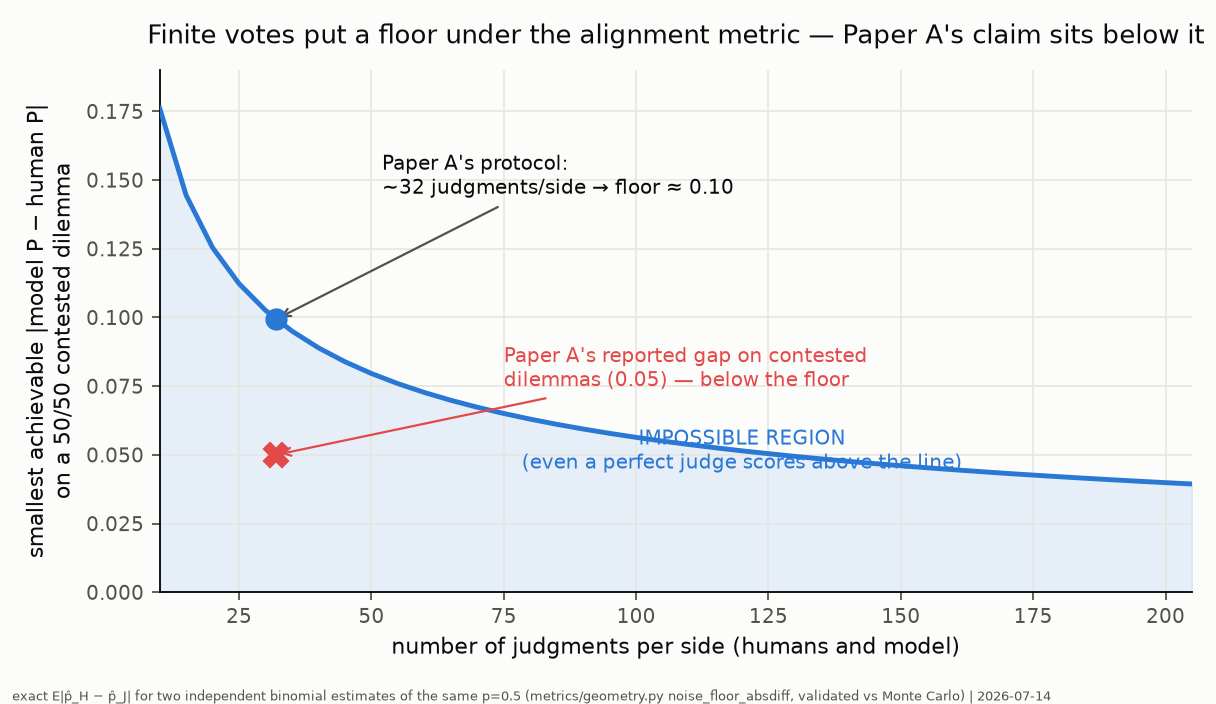
\includegraphics[width=0.72\linewidth]{finding4_noise-floor-vs-n_paperA-claim_2026-07-14.png}
  \caption{The smallest distribution gap a perfect judge can score, by number of votes per side. The reported contested-item gap of \citet{russo2026pluralistic} sits below the floor of its own protocol.}
  \label{fig:floor}
\end{figure}

\section{Discussion}

Both papers' \emph{diagnoses} survive our scrutiny. We reproduce the value-collapse number almost exactly (0.80 vs.\ their 0.82, different model and pipeline), and model judges do agree with each other ($r=0.60$) more than humans agree with humans (0.45), and more than they agree with humans (0.38). What fails is the cure, and the metrics that certified it. Persona conditioning is a variance dial. Distribution and diversity metrics read variance as pluralism; direction metrics do not, and direction does not move---not for prompting (this paper), and not for fine-tuning \citep{mukherjee2026geometry}. That two entirely different intervention classes fail identically suggests the judge--human gap lives somewhere conditioning cannot reach.

The constructive findings are almost embarrassingly simple. If you need distributional answers, ask distributional questions. If you need a judge more aligned with people, use a better model. And if you evaluate a pluralism intervention, require it to beat a scrambled-content control and a matched-noise null before its diversity numbers count.

\section{Limitations}

One moral domain (AITA) plus one multilingual evaluation domain (PARIKSHA); moral ground truth is English-speaking, self-selected Reddit commenters, so our claims are about matching \emph{this} population, not humanity; judges saw abstracted rewrites while the humans voted on originals (identical across conditions, so contrasts are clean, but absolute gaps are inflated); seven judges from four model families; the geometry paper's headline dataset is private and its angle estimator unspecified, so our reproduction commits to a pre-registered operationalization on the public half; value extraction from rationales uses a single LLM extractor; all human rates carry the finite-vote floors we report.

\section*{Broader impact}

This paper argues against deploying persona-conditioned LLM judges as stand-ins for diverse human judgment, and against trusting diversity metrics as evidence of pluralism. Both points reduce, rather than create, risk of overclaiming in evaluation pipelines. All human data used is public and de-identified; dilemma texts are abstracted retellings to prevent traceability.

\section*{Reproducibility}

The released repository \emph{(TODO: anonymized link)} contains the pre-registrations (committed before each phase), all prompts and conditions, the unit-tested metrics library, 75k+ raw judgments with per-row labels, spend logs, and per-figure provenance.

\bibliographystyle{plainnat}
\bibliography{refs}

\end{document}
